% ============================================================================
% CHƯƠNG III: CÀI ĐẶT VÀ ĐÁNH GIÁ HỆ THỐNG
% ============================================================================
\chapter{CÀI ĐẶT VÀ ĐÁNH GIÁ HỆ THỐNG}

\section{Hướng dẫn cài đặt và khởi động hệ thống}

\subsection{Yêu cầu hệ thống}

\begin{table}[H]
\centering
\caption{Yêu cầu phần mềm}
\begin{tabular}{|l|l|l|}
\hline
\textbf{Phần mềm} & \textbf{Phiên bản} & \textbf{Ghi chú} \\
\hline
PHP & 8.4+ & Với MongoDB extension \\
Composer & 2.x & Package manager \\
Docker & 20.x+ & Container runtime \\
Docker Compose & 2.x & Multi-container \\
MongoDB Compass & 1.40+ & GUI (optional) \\
\hline
\end{tabular}
\end{table}

\subsection{Khởi động hệ thống với script tự động}

Hệ thống cung cấp script \texttt{start\_system.sh} để khởi động một cách tự động:

\begin{lstlisting}[language=bash, caption=start\_system.sh - Khởi động hệ thống]
#!/usr/bin/env bash
echo "=== KHOI DONG E-LIBRARY SYSTEM ==="

# Step 1: Check Docker
if ! docker ps >/dev/null 2>&1; then
    echo "LOI: Docker chua chay!"
    exit 1
fi

# Step 2: Start MongoDB Replica Set
MONGO_COUNT=$(docker ps | grep -c mongo || echo "0")
if [ "$MONGO_COUNT" -lt 1 ]; then
    docker-compose up -d
    sleep 10
fi

# Step 3: Verify MongoDB connection
docker exec mongo1 mongosh --quiet --eval "db.version()"

# Step 4: Start PHP server
cd Nhasach
php -S localhost:8000 &

echo "=== HE THONG DA SAN SANG! ==="
echo "URL: http://localhost:8000"
echo "Login: admin / 123456"
\end{lstlisting}

\section{Các công cụ sử dụng cài đặt hệ thống}

\subsection{MongoDB 4.4 và MongoDB Compass}

MongoDB phiên bản 4.4 được triển khai qua Docker image chính thức. MongoDB Compass phiên bản 1.40+ được sử dụng để:

\begin{enumerate}
    \item \textbf{Schema Visualization}: Phân tích cấu trúc documents tự động
    \item \textbf{Aggregation Pipeline Builder}: Xây dựng pipeline với giao diện drag-and-drop
    \item \textbf{Explain Plan}: Phân tích query execution, index usage
    \item \textbf{Real-time Performance}: Theo dõi operations/second, connections
\end{enumerate}

\subsection{PHP 8.4 và MongoDB Driver}

Cấu hình kết nối MongoDB hỗ trợ 3 chế độ: standalone, replicaset, và sharded:

\begin{lstlisting}[language=PHP, caption=Connection.php - Đầy đủ 3 mode kết nối]
<?php
require 'vendor/autoload.php';
use MongoDB\Client;

$MODE = 'sharded'; // Options: standalone, replicaset, sharded
$Database = "Nhasach";

try {
    switch ($MODE) {
        case 'sharded':
            // Via mongos router
            $conn = new Client("mongodb://localhost:27017", [
                'readPreference' => 'primaryPreferred',
                'w' => 'majority',
                'journal' => true
            ]);
            break;

        case 'replicaset':
            // Direct to replica set
            $conn = new Client(
                "mongodb://mongo1:27017,mongo2:27017,mongo3:27017/?replicaSet=rs0",
                ['readPreference' => 'primaryPreferred', 'w' => 'majority']
            );
            break;

        default:
            // Standalone
            $conn = new Client("mongodb://localhost:27017");
    }
    $db = $conn->$Database;
} catch (Exception $e) {
    die("Khong the ket noi MongoDB: " . $e->getMessage());
}
\end{lstlisting}

\subsection{Docker Compose cho MongoDB Replica Set}

Cấu hình Docker Compose với 3 MongoDB containers:

\begin{lstlisting}[caption=docker-compose.yml - MongoDB Replica Set đầy đủ]
version: '3.8'

services:
  mongo1:
    image: mongo:4.4
    container_name: mongo1
    hostname: mongo1
    ports:
      - "27017:27017"
    environment:
      - MONGO_INITDB_DATABASE=Nhasach
    volumes:
      - mongo1_data:/data/db
    networks:
      mongo-net:
        aliases: [mongo1]
    command: ["mongod", "--replSet", "rs0", "--bind_ip_all"]
    restart: unless-stopped

  mongo2:
    image: mongo:4.4
    container_name: mongo2
    ports: ["27018:27017"]
    volumes: [mongo2_data:/data/db]
    networks: [mongo-net]
    command: ["mongod", "--replSet", "rs0", "--bind_ip_all"]
    depends_on: [mongo1]

  mongo3:
    image: mongo:4.4
    container_name: mongo3
    ports: ["27019:27017"]
    volumes: [mongo3_data:/data/db]
    networks: [mongo-net]
    command: ["mongod", "--replSet", "rs0", "--bind_ip_all"]
    depends_on: [mongo1]

networks:
  mongo-net:
    driver: bridge

volumes:
  mongo1_data:
    name: elibrary_mongo1_data
  mongo2_data:
    name: elibrary_mongo2_data
  mongo3_data:
    name: elibrary_mongo3_data
\end{lstlisting}

\section{Một số giao diện chính của hệ thống}

\subsection{Giao diện đăng nhập}

\begin{figure}[H]
    \centering
    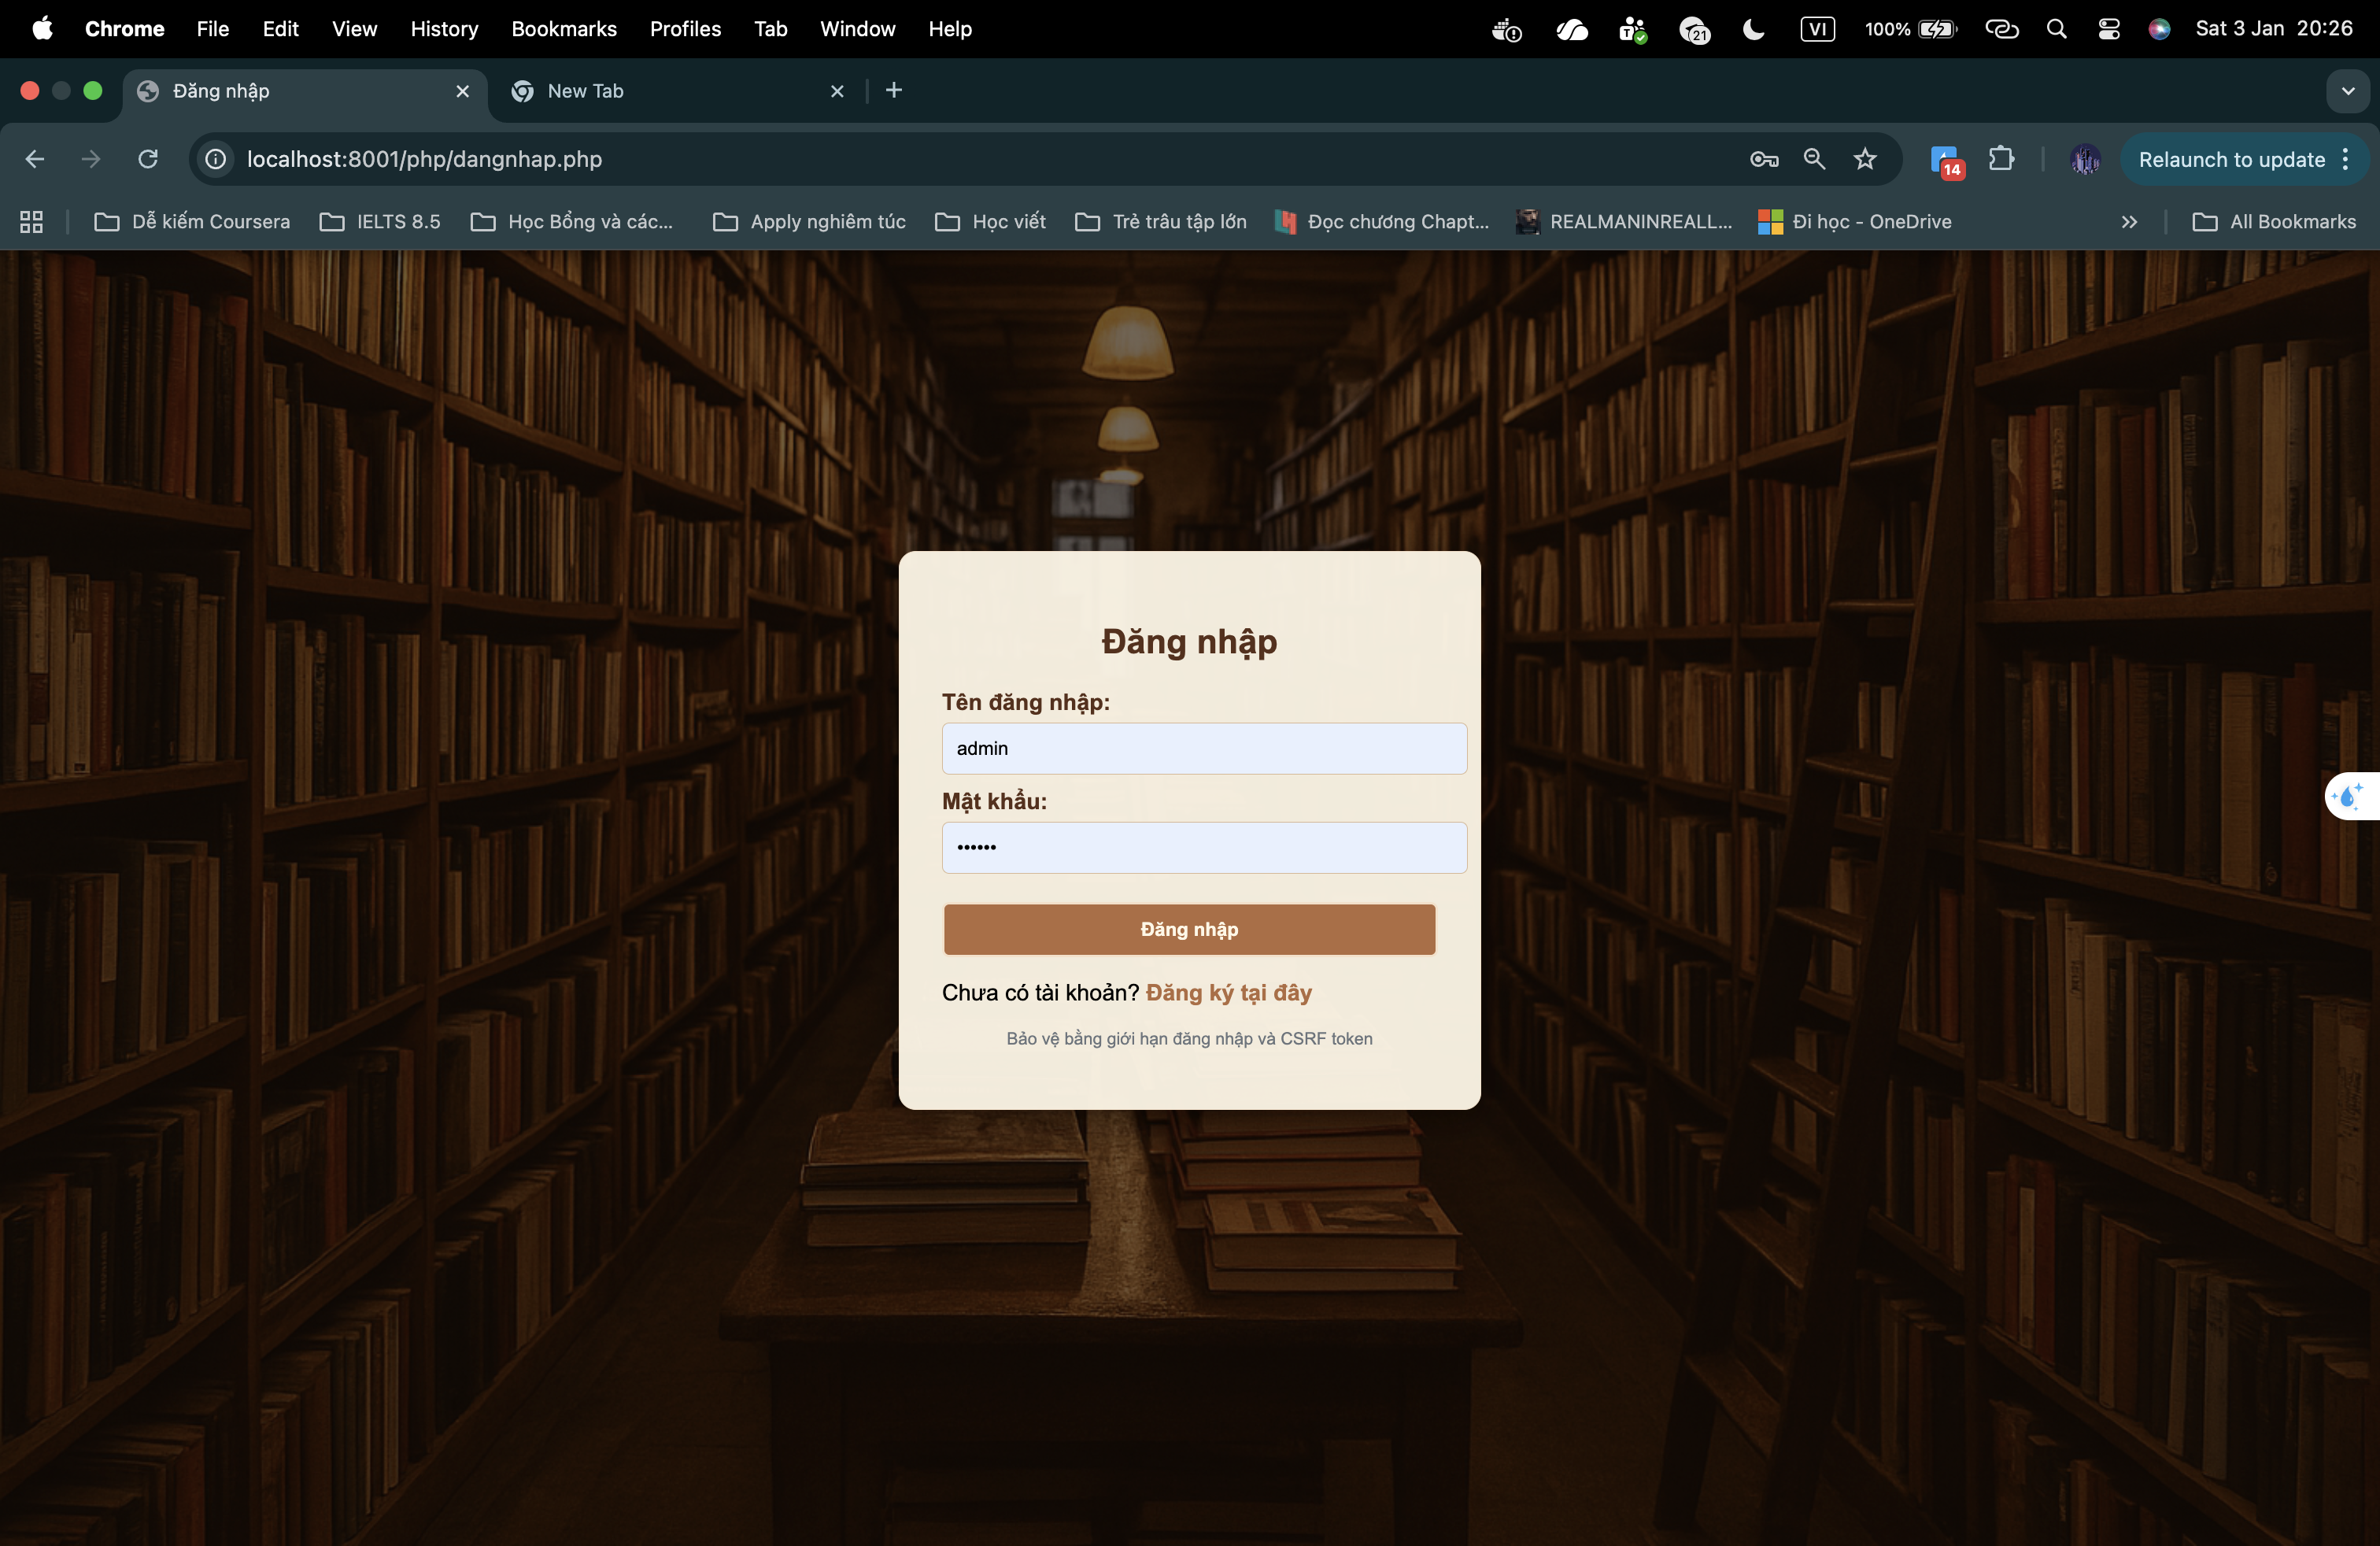
\includegraphics[width=0.85\textwidth]{01_login.png}
    \caption{Giao diện đăng nhập hệ thống}
    \label{fig:login}
\end{figure}

Giao diện đăng nhập hỗ trợ:
\begin{itemize}
    \item Xác thực username/password với bcrypt hash
    \item Phát hiện brute-force attack (lock sau 5 lần thất bại)
    \item Tạo JWT token với thời hạn 24 giờ
    \item Chuyển hướng theo role (admin $\rightarrow$ dashboard, customer $\rightarrow$ danhsachsach)
\end{itemize}

\subsection{Dashboard thống kê (Admin)}

\begin{figure}[H]
    \centering
    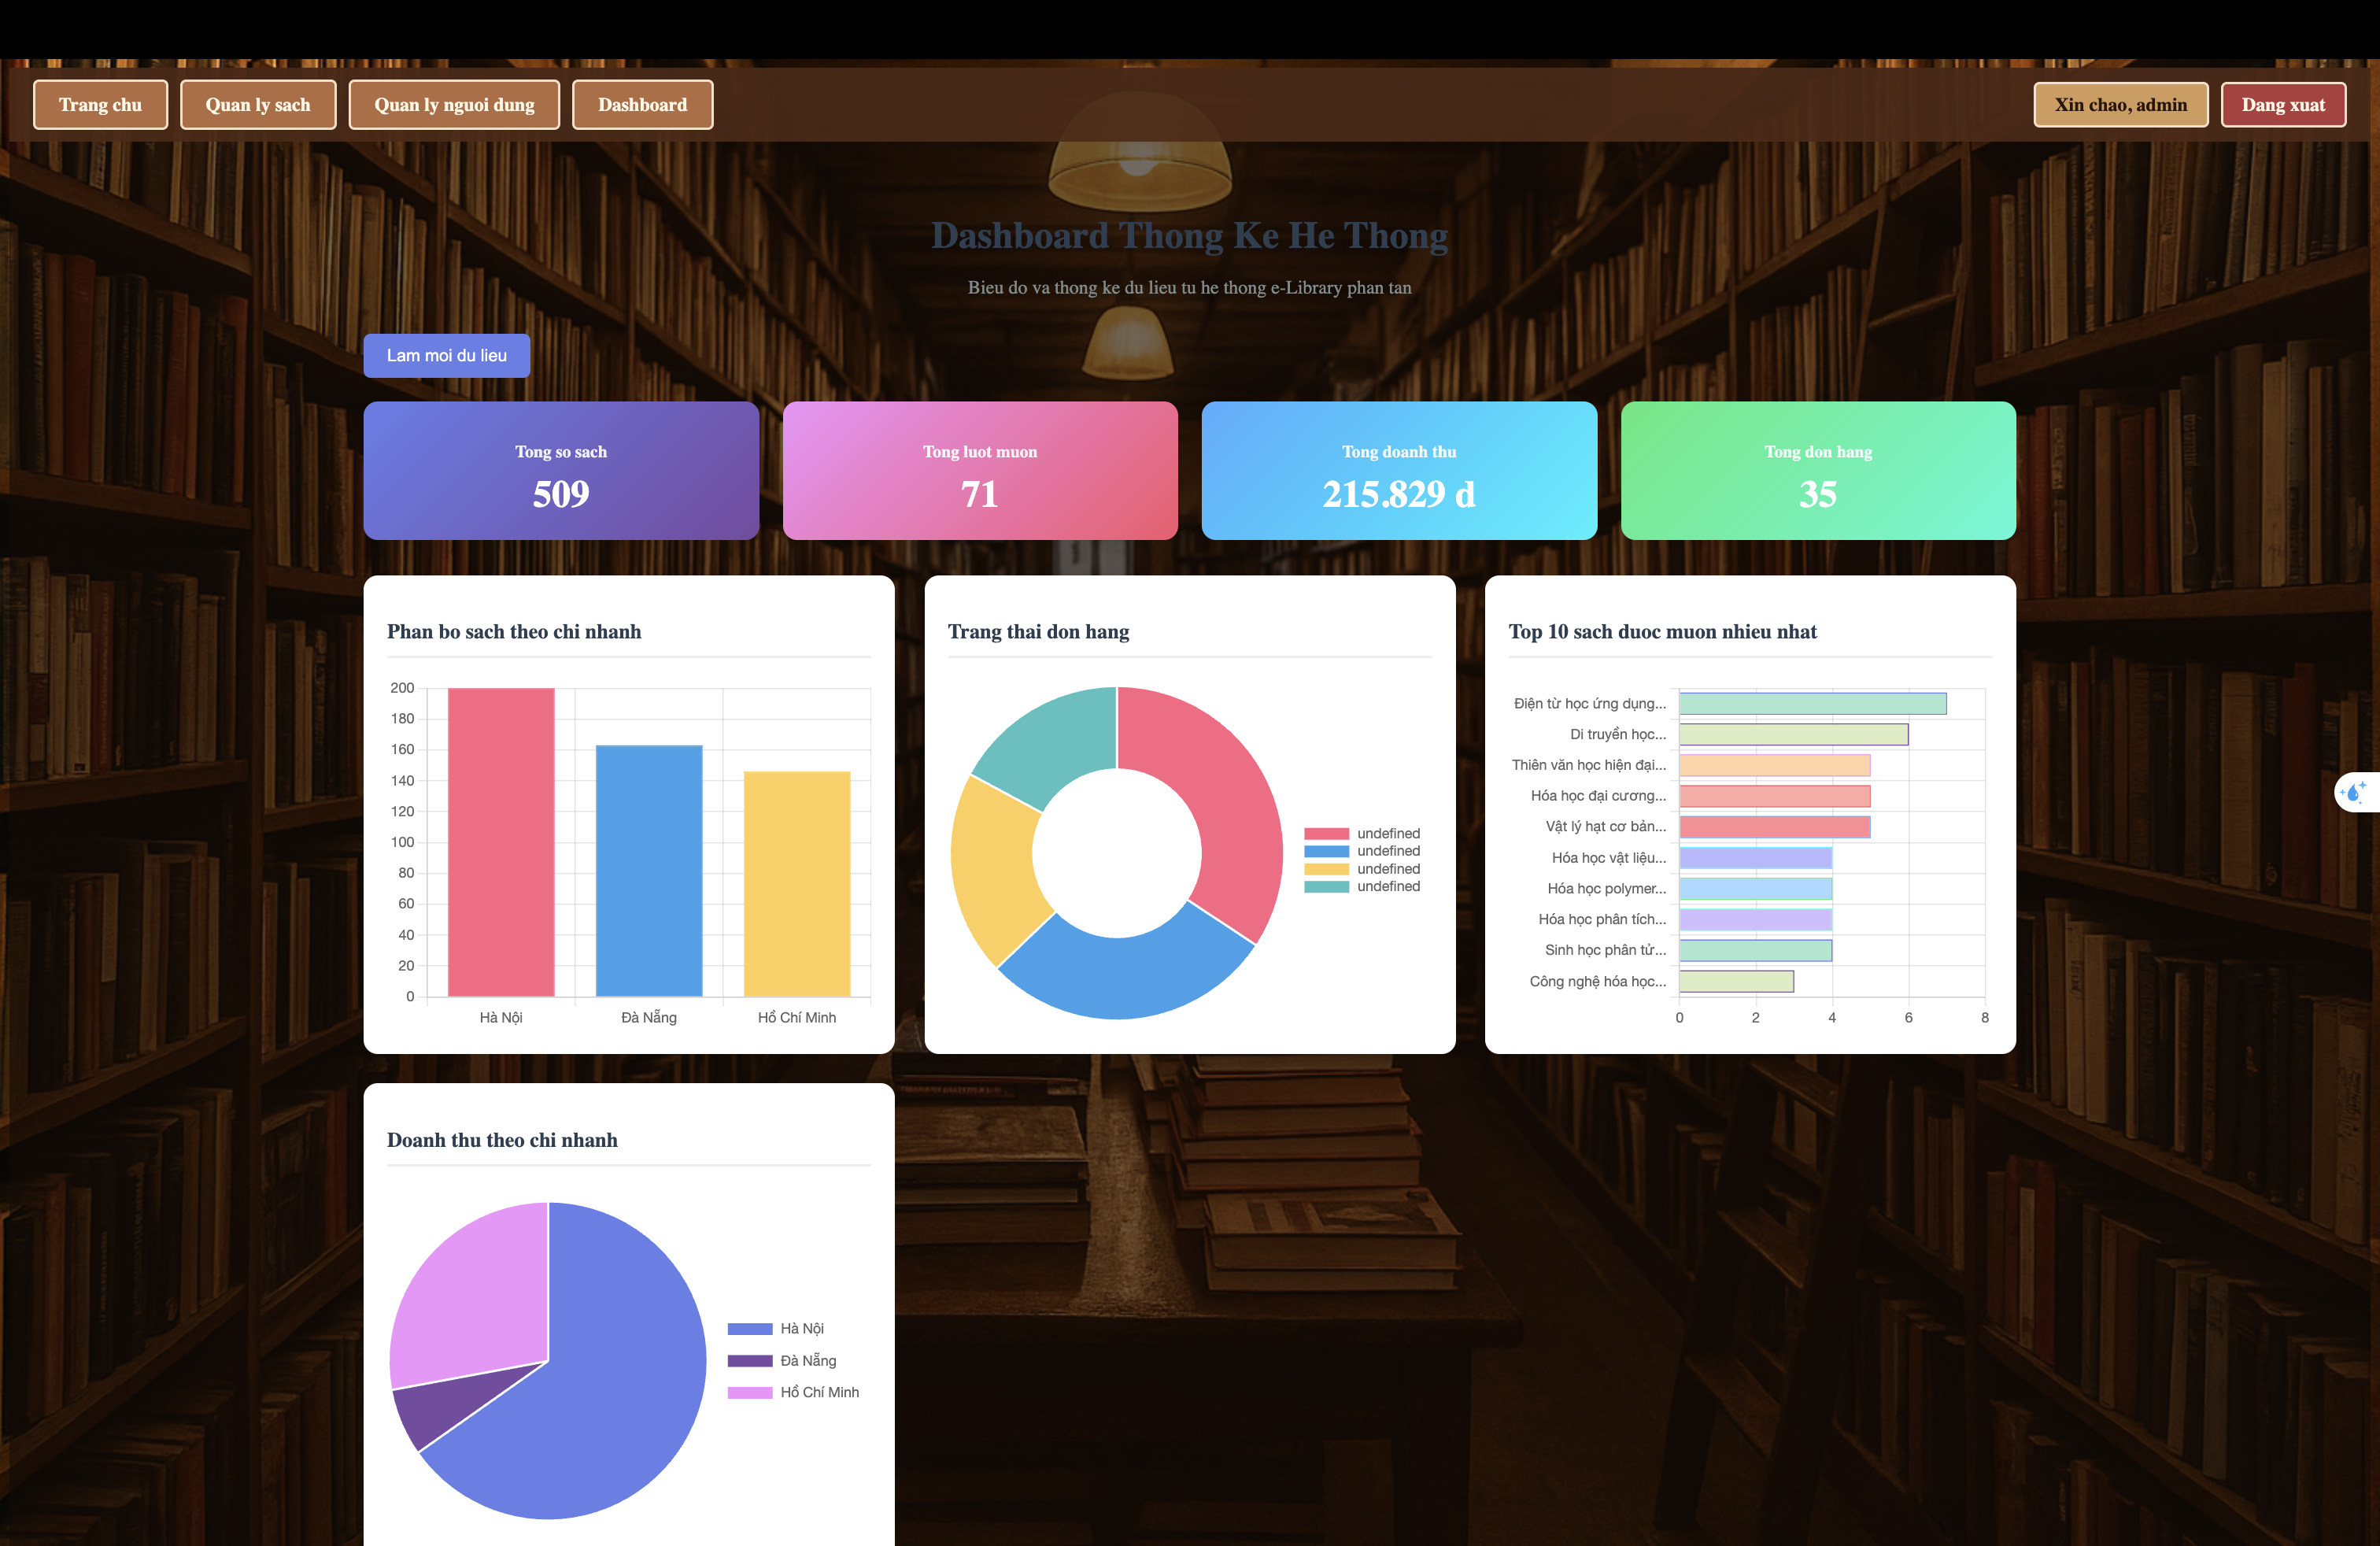
\includegraphics[width=\textwidth]{02_dashboard.png}
    \caption{Dashboard thống kê với biểu đồ Chart.js}
    \label{fig:dashboard}
\end{figure}

Dashboard hiển thị:
\begin{itemize}
    \item Tổng số sách, người dùng, đơn mượn qua cards
    \item Biểu đồ cột: Sách theo chi nhánh
    \item Biểu đồ tròn: Trạng thái đơn hàng
    \item Dữ liệu lấy từ API \texttt{/api/statistics.php}
\end{itemize}

\subsection{Quản lý sách (Admin)}

\begin{figure}[H]
    \centering
    \includegraphics[width=\textwidth]{03_quanlysach.png}
    \caption{Giao diện CRUD quản lý sách}
    \label{fig:quanlysach}
\end{figure}

\subsection{Danh sách sách (Customer)}

\begin{figure}[H]
    \centering
    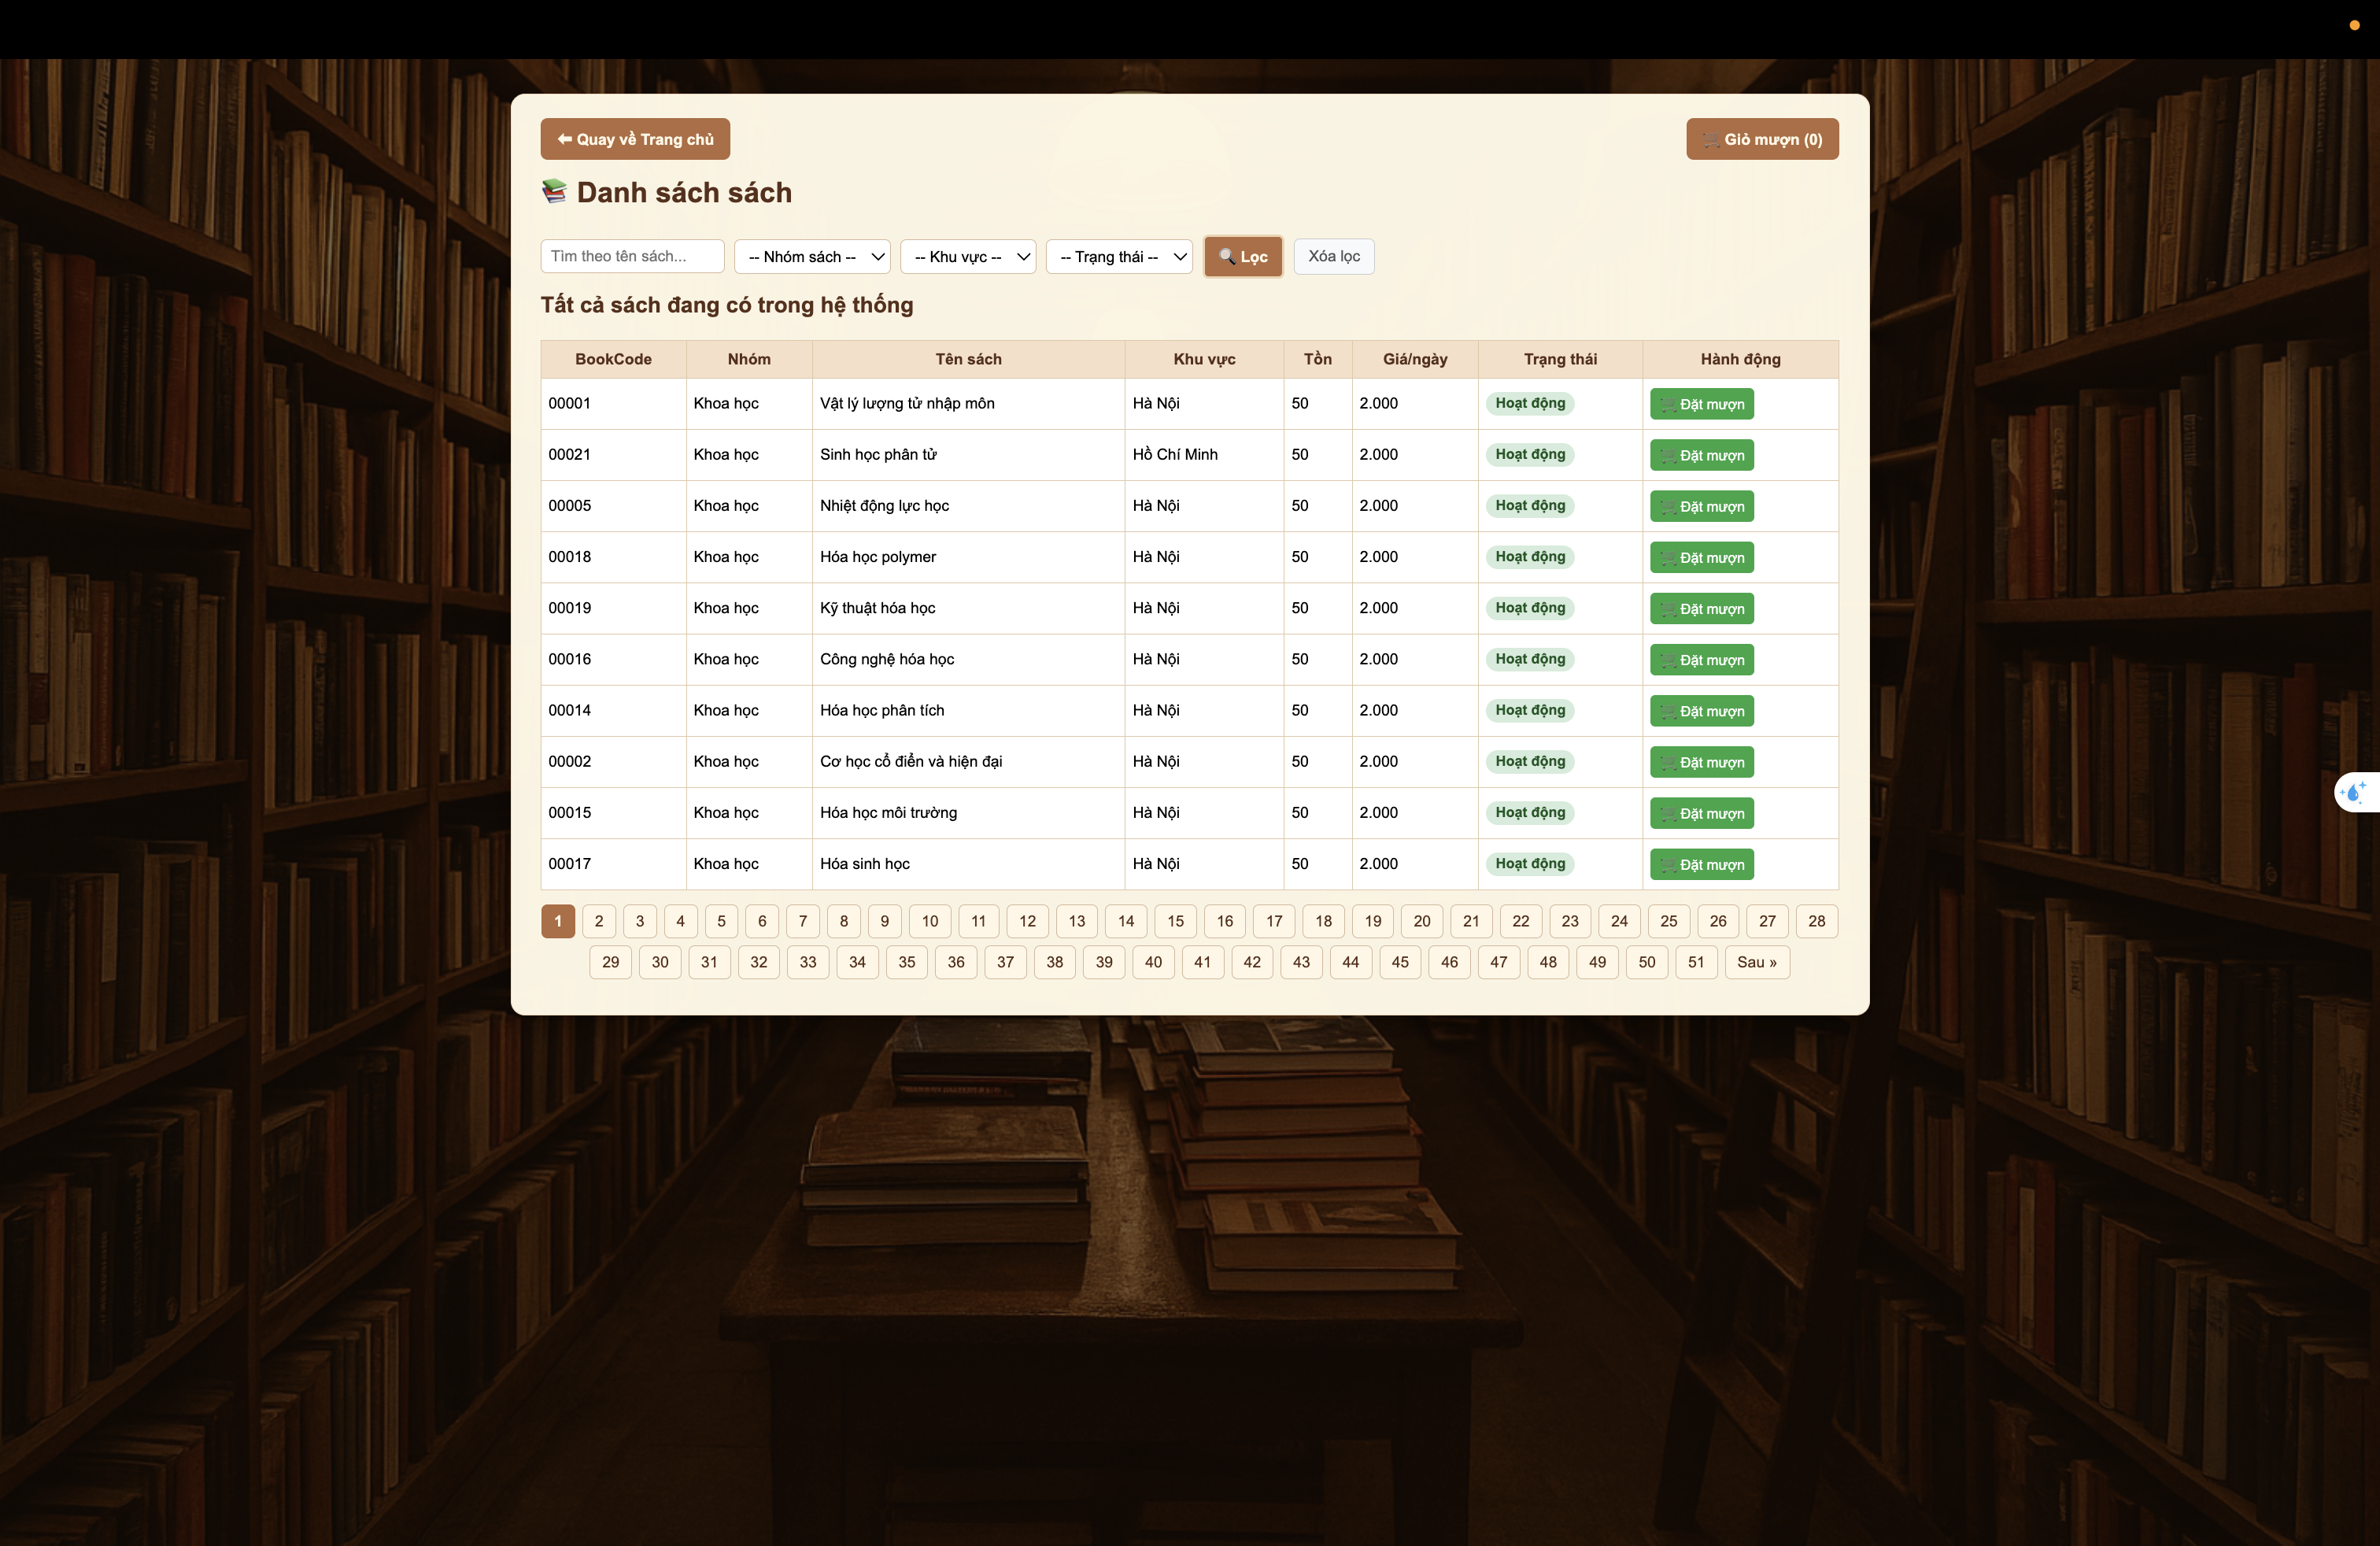
\includegraphics[width=\textwidth]{05_danhsachsach.png}
    \caption{Danh sách sách cho khách hàng}
    \label{fig:danhsachsach}
\end{figure}

\subsection{Giỏ hàng mượn sách}

\begin{figure}[H]
    \centering
    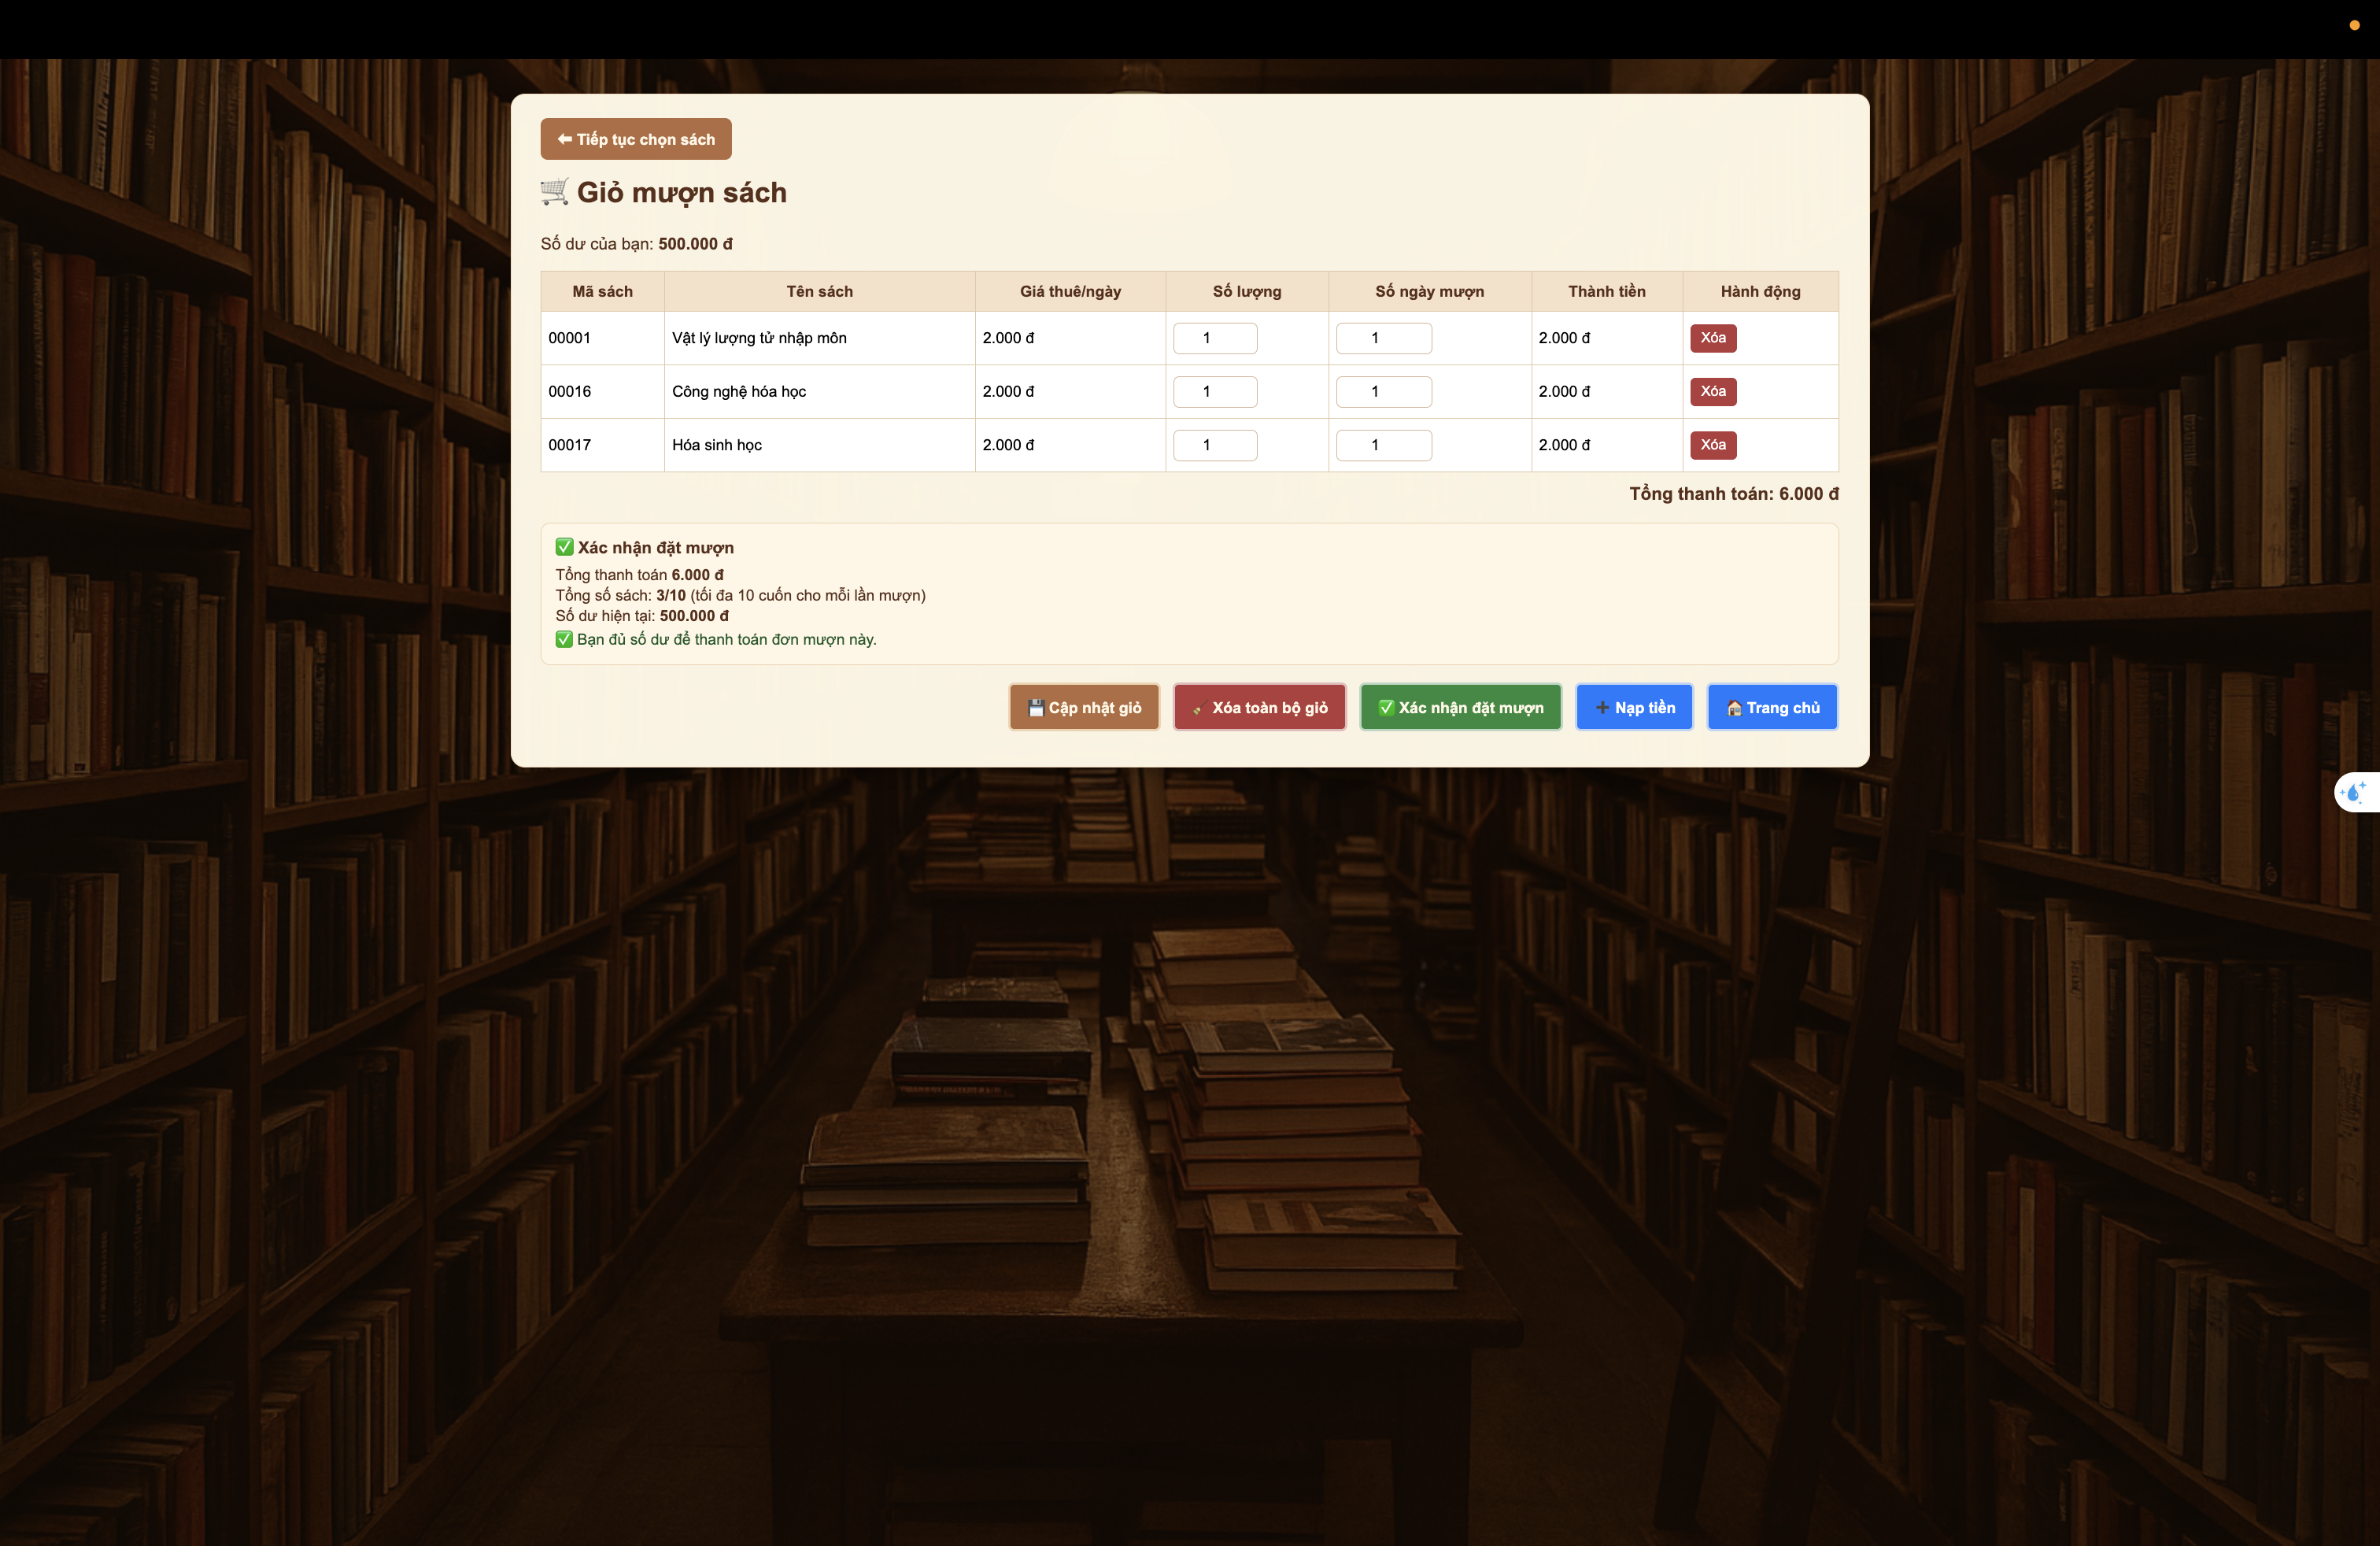
\includegraphics[width=\textwidth]{06_giohang.png}
    \caption{Giao diện giỏ hàng mượn sách}
    \label{fig:giohang}
\end{figure}

\subsection{Docker Containers}

\begin{figure}[H]
    \centering
    \includegraphics[width=0.8\textwidth]{10_docker.png}
    \caption{Docker Desktop hiển thị MongoDB containers}
    \label{fig:docker}
\end{figure}

\subsection{MongoDB Compass}

\begin{figure}[H]
    \centering
    \includegraphics[width=\textwidth]{11_mongodb_compass.png}
    \caption{MongoDB Compass hiển thị collection books}
    \label{fig:compass}
\end{figure}

\section{Triển khai Aggregation Pipeline}

\subsection{Tổng quan API Statistics}

Hệ thống cung cấp 8 endpoints thống kê sử dụng Aggregation Pipeline trong file \texttt{api/statistics.php}:

\begin{table}[H]
\centering
\caption{Danh sách Aggregation Pipeline endpoints}
\begin{tabular}{|c|l|l|}
\hline
\textbf{\#} & \textbf{Action} & \textbf{Pipeline Stages} \\
\hline
1 & books\_by\_location & \$match, \$group, \$sort, \$project \\
2 & popular\_books & \$match, \$sort, \$limit, \$project \\
3 & revenue\_by\_date & \$match, \$addFields, \$group, \$sort, \$project \\
4 & user\_statistics & \$match, \$group, \$sort, \$limit, \$addFields, \$project \\
5 & user\_details & \$match, \textbf{\$lookup}, \$unwind, \$group, \$sort, \$limit \\
6 & order\_status\_summary & \$group, \$sort, \$project \\
7 & monthly\_trends & \$match, \$addFields, \$group, \$sort, \$project \\
8 & book\_group\_stats & \$match, \textbf{\$facet}, \textbf{\$bucket} \\
\hline
\end{tabular}
\end{table}

\subsection{Endpoint books\_by\_location}

\begin{lstlisting}[language=PHP, caption=statistics.php - books\_by\_location với 4 stages]
case 'books_by_location':
    $pipeline = [
        // Stage 1: $match - Filter active books
        ['$match' => ['status' => ['$ne' => 'deleted']]],

        // Stage 2: $group - Aggregate by location
        ['$group' => [
            '_id' => '$location',
            'totalBooks' => ['$sum' => 1],
            'totalQuantity' => ['$sum' => '$quantity'],
            'avgPricePerDay' => ['$avg' => '$pricePerDay'],
            'totalBorrowCount' => ['$sum' => '$borrowCount']
        ]],

        // Stage 3: $sort - Order by total books
        ['$sort' => ['totalBooks' => -1]],

        // Stage 4: $project - Rename and format fields
        ['$project' => [
            '_id' => 0,
            'location' => '$_id',
            'totalBooks' => 1,
            'totalQuantity' => 1,
            'avgPricePerDay' => ['$round' => ['$avgPricePerDay', 0]],
            'totalBorrowCount' => 1
        ]]
    ];

    $result = $db->books->aggregate($pipeline)->toArray();
\end{lstlisting}

\subsection{Endpoint user\_details với \$lookup JOIN}

Đây là endpoint quan trọng nhất, thể hiện khả năng JOIN giữa các collections trong MongoDB:

\begin{lstlisting}[language=PHP, caption=statistics.php - user\_details với \$lookup]
case 'user_details':
    $pipeline = [
        // Stage 1: Match completed orders
        ['$match' => ['status' => ['$in' => ['paid', 'success', 'returned']]]],

        // Stage 2: $lookup - LEFT OUTER JOIN with users collection
        ['$lookup' => [
            'from' => 'users',           // Target collection
            'localField' => 'user_id',   // Field in orders
            'foreignField' => '_id',     // Field in users
            'as' => 'user_info'          // Output array
        ]],

        // Stage 3: $unwind - Flatten user_info array
        ['$unwind' => [
            'path' => '$user_info',
            'preserveNullAndEmptyArrays' => true
        ]],

        // Stage 4: Group by user with joined info
        ['$group' => [
            '_id' => '$user_id',
            'username' => ['$first' => '$username'],
            'email' => ['$first' => '$user_info.email'],
            'fullname' => ['$first' => '$user_info.fullname'],
            'role' => ['$first' => '$user_info.role'],
            'totalOrders' => ['$sum' => 1],
            'totalSpent' => ['$sum' => '$total_amount']
        ]],

        ['$sort' => ['totalSpent' => -1]],
        ['$limit' => 20]
    ];

    $result = $db->orders->aggregate($pipeline)->toArray();
\end{lstlisting}

\subsection{Endpoint book\_group\_stats với \$facet và \$bucket}

\begin{lstlisting}[language=PHP, caption=statistics.php - Multi-faceted statistics]
case 'book_group_stats':
    $pipeline = [
        ['$match' => ['status' => ['$ne' => 'deleted']]],

        ['$facet' => [
            // Facet 1: Statistics by book group
            'byGroup' => [
                ['$group' => [
                    '_id' => '$bookGroup',
                    'count' => ['$sum' => 1],
                    'totalQuantity' => ['$sum' => '$quantity']
                ]],
                ['$sort' => ['count' => -1]]
            ],

            // Facet 2: Overall summary
            'summary' => [
                ['$group' => [
                    '_id' => null,
                    'totalBooks' => ['$sum' => 1],
                    'avgPrice' => ['$avg' => '$pricePerDay'],
                    'totalBorrows' => ['$sum' => '$borrowCount']
                ]]
            ],

            // Facet 3: Price distribution with $bucket
            'priceRanges' => [
                ['$bucket' => [
                    'groupBy' => '$pricePerDay',
                    'boundaries' => [0, 5000, 10000, 20000, 50000, 100000],
                    'default' => 'Other',
                    'output' => ['count' => ['$sum' => 1]]
                ]]
            ]
        ]]
    ];
\end{lstlisting}

\section{Triển khai Map-Reduce}

\subsection{Tổng quan API Map-Reduce}

File \texttt{api/mapreduce.php} cung cấp 5 Map-Reduce operations:

\begin{table}[H]
\centering
\caption{Danh sách Map-Reduce operations}
\begin{tabular}{|c|l|l|}
\hline
\textbf{\#} & \textbf{Action} & \textbf{Mô tả} \\
\hline
1 & borrow\_stats & Thống kê mượn sách theo bookCode \\
2 & revenue\_by\_user & Doanh thu theo user \\
3 & books\_by\_category & Sách theo thể loại \\
4 & daily\_activity & Hoạt động theo ngày \\
5 & location\_performance & Hiệu suất theo chi nhánh \\
\hline
\end{tabular}
\end{table}

\subsection{Map-Reduce: borrow\_stats}

\begin{lstlisting}[language=PHP, caption=mapreduce.php - Borrowing statistics]
case 'borrow_stats':
    // Map function: emit bookCode with borrow info
    $mapFunction = new MongoDB\BSON\Javascript('
        function() {
            if (this.items && Array.isArray(this.items)) {
                for (var i = 0; i < this.items.length; i++) {
                    var item = this.items[i];
                    emit(item.bookCode, {
                        count: 1,
                        quantity: item.quantity || 1,
                        revenue: item.subtotal || 0,
                        bookName: item.bookName || "Unknown"
                    });
                }
            }
        }
    ');

    // Reduce function: aggregate values
    $reduceFunction = new MongoDB\BSON\Javascript('
        function(key, values) {
            var result = { count: 0, quantity: 0, revenue: 0, bookName: "" };
            for (var i = 0; i < values.length; i++) {
                result.count += values[i].count;
                result.quantity += values[i].quantity;
                result.revenue += values[i].revenue;
                if (values[i].bookName !== "Unknown") {
                    result.bookName = values[i].bookName;
                }
            }
            return result;
        }
    ');

    // Finalize function: calculate averages
    $finalizeFunction = new MongoDB\BSON\Javascript('
        function(key, reducedValue) {
            reducedValue.avgQuantityPerOrder = reducedValue.count > 0
                ? reducedValue.quantity / reducedValue.count : 0;
            return reducedValue;
        }
    ');

    $result = $db->command([
        'mapReduce' => 'orders',
        'map' => $mapFunction,
        'reduce' => $reduceFunction,
        'finalize' => $finalizeFunction,
        'out' => ['inline' => 1],
        'query' => ['status' => ['$in' => ['paid', 'success', 'returned']]]
    ]);
\end{lstlisting}

\section{Kiểm thử hệ thống}

\subsection{Kịch bản 1: Kiểm thử hiển thị dữ liệu}

\textbf{Mục đích:} Đảm bảo dữ liệu hiển thị đúng tại mỗi chi nhánh.

\textbf{Kết quả:}
\begin{table}[H]
\centering
\caption{Kết quả kiểm thử hiển thị dữ liệu}
\begin{tabular}{|l|c|c|c|c|}
\hline
\textbf{Chi nhánh} & \textbf{Port} & \textbf{Books} & \textbf{Users} & \textbf{Orders} \\
\hline
Central Hub & 8001 & 509 & 2 & 0 \\
Hà Nội & 8002 & 162 & 13 & 46 \\
Đà Nẵng & 8003 & 127 & 12 & 0 \\
TP.HCM & 8004 & 111 & 11 & 0 \\
\hline
\end{tabular}
\end{table}

\textbf{Đánh giá:} \textcolor{green}{PASS} - Dữ liệu hiển thị đúng theo từng database.

\subsection{Kịch bản 2: Kiểm thử ghi và đồng bộ}

\textbf{Mục đích:} Đảm bảo dữ liệu đồng bộ từ PRIMARY sang SECONDARY.

\textbf{Các bước:}
\begin{enumerate}
    \item Thêm sách mới tại Central Hub
    \item Kiểm tra sách xuất hiện tại mongo2, mongo3
    \item Đo replication lag
\end{enumerate}

\textbf{Kết quả:}
\begin{itemize}
    \item Ghi vào PRIMARY: Thành công
    \item Replication lag: 50-200ms
    \item Dữ liệu nhất quán: OK
\end{itemize}

\textbf{Đánh giá:} \textcolor{green}{PASS}

\subsection{Kịch bản 3: Kiểm thử Failover}

\textbf{Mục đích:} Đảm bảo hệ thống tự động phục hồi khi PRIMARY gặp sự cố.

\textbf{Các bước:}
\begin{lstlisting}[language=bash, caption=Script kiểm thử Failover]
# 1. Check current status
docker exec mongo1 mongosh --eval "rs.status().members.map(m => m.stateStr)"

# 2. Stop PRIMARY
docker stop mongo1

# 3. Wait for election (10-15s)
sleep 15

# 4. Check new PRIMARY
docker exec mongo2 mongosh --eval "rs.status().members.map(m => m.stateStr)"

# 5. Restart old PRIMARY
docker start mongo1
\end{lstlisting}

\textbf{Kết quả:}
\begin{itemize}
    \item Phát hiện node hỏng: $\sim$10 giây
    \item Bầu chọn PRIMARY mới: $\sim$5 giây
    \item Tổng thời gian gián đoạn: \textbf{10-15 giây}
    \item Hệ thống tiếp tục hoạt động: OK
\end{itemize}

\textbf{Đánh giá:} \textcolor{green}{PASS}

\subsection{Kịch bản 4: Benchmark hiệu năng}

Benchmark được thực hiện với \textbf{50 iterations} mỗi test case trên MongoDB 8.0.16:

\begin{figure}[H]
    \centering
    \includegraphics[width=\textwidth]{12_terminal_benchmark.png}
    \caption{Kết quả benchmark trong Terminal}
    \label{fig:benchmark}
\end{figure}

\begin{table}[H]
\centering
\caption{Kết quả benchmark hiệu năng (REAL DATA)}
\label{tab:benchmark}
\begin{tabular}{|l|c|c|c|}
\hline
\textbf{Test Case} & \textbf{Avg (ms)} & \textbf{Total (ms)} & \textbf{Ops/Sec} \\
\hline
Compound Query (location+bookGroup) & \textbf{0.300} & 15 & 3,333 \\
Point Lookup (bookCode) & 0.420 & 21 & 2,381 \\
Update Operation (\$inc + \$set) & 0.480 & 24 & 2,083 \\
Text Search & 0.640 & 32 & 1,563 \\
Range Query + Sort & 0.820 & 41 & 1,220 \\
Write (Insert + Delete) & 1.120 & 56 & 893 \\
Aggregation (\$group) & 1.820 & 91 & 549 \\
Single Location Query & 1.980 & 99 & 505 \\
Cross-Shard Query & 2.380 & 119 & 420 \\
Complex Aggregation (\$facet) & \textbf{3.080} & 154 & 325 \\
\hline
\end{tabular}
\end{table}

\textbf{Phân tích:}
\begin{itemize}
    \item \textbf{Fastest}: Compound Query 0.300ms - Index prefix matching hiệu quả
    \item \textbf{Slowest}: \$facet 3.080ms - 3 parallel sub-pipelines
    \item \textbf{Average}: 1.304ms - Đạt yêu cầu < 3ms
    \item \textbf{Peak Throughput}: 3,333 ops/sec
\end{itemize}

\section{Đánh giá hệ thống}

\subsection{Ưu điểm}

\begin{enumerate}
    \item \textbf{Tính sẵn sàng cao (High Availability)}:
    \begin{itemize}
        \item Replica Set 3 nodes đảm bảo hoạt động khi 1 node gặp sự cố
        \item Automatic failover trong 10-15 giây
        \item Read Preference: primaryPreferred cho read availability
    \end{itemize}

    \item \textbf{Hiệu năng tốt}:
    \begin{itemize}
        \item Query trung bình 1.304ms
        \item Compound index với partition key cho query < 1ms
        \item TEXT index cho full-text search 0.640ms
    \end{itemize}

    \item \textbf{Aggregation Pipeline mạnh mẽ}:
    \begin{itemize}
        \item 8 endpoints với 10+ operators
        \item \$lookup cho JOIN giữa collections
        \item \$facet cho multi-faceted analysis
    \end{itemize}

    \item \textbf{Bảo mật đầy đủ}:
    \begin{itemize}
        \item JWT authentication với expiration 24h
        \item bcrypt password hashing (cost 12)
        \item RBAC: admin vs customer
    \end{itemize}
\end{enumerate}

\subsection{Nhược điểm và Hạn chế}

\begin{enumerate}
    \item \textbf{Shard Key Cardinality thấp}:
    \begin{itemize}
        \item location chỉ có 3 giá trị
        \item Có thể gây jumbo chunks khi scale
        \item Khuyến nghị: Compound shard key \{location: 1, bookCode: 1\}
    \end{itemize}

    \item \textbf{Dataset thử nghiệm nhỏ}:
    \begin{itemize}
        \item 909 sách chưa đủ stress test
        \item Chunk migration chưa được trigger
    \end{itemize}

    \item \textbf{Chưa có TLS/SSL}:
    \begin{itemize}
        \item Kết nối MongoDB chưa mã hóa
        \item Cần bổ sung cho production
    \end{itemize}

    \item \textbf{Phức tạp vận hành}:
    \begin{itemize}
        \item Cần quản lý 3+ Docker containers
        \item Monitoring đa node
    \end{itemize}
\end{enumerate}

\subsection{So sánh với các hệ thống khác}

\begin{table}[H]
\centering
\caption{So sánh MongoDB với các hệ thống phân tán khác}
\begin{tabular}{|l|c|c|c|}
\hline
\textbf{Tiêu chí} & \textbf{MongoDB} & \textbf{Cassandra} & \textbf{PostgreSQL} \\
\hline
CAP Theorem & CP/AP & AP & CP \\
Consistency & Tunable & Eventual & Strong \\
Aggregation & Excellent & Limited & Good \\
Scaling & Horizontal & Horizontal & Vertical \\
Learning Curve & Medium & High & Low \\
\hline
\end{tabular}
\end{table}

MongoDB được chọn vì:
\begin{itemize}
    \item Aggregation Pipeline mạnh mẽ cho Dashboard
    \item Flexible schema cho rapid development
    \item Mature PHP driver và ecosystem
\end{itemize}
